\section{Methodology}
\label{sec:methodology}

Hyperbolic spaces are more suitable for embedding hierarchical relationships with low distortion \citep{Sarkar_2012} and low dimensions. Hence, motivated by the aforementioned challenges, we propose a \textbf{Hyp}erbolic \textbf{Structure}d regularizer for \emph{hierarchy-informed} representation learning. We begin with the basics of hyperbolic geometry, followed by the detailed methodology of our proposed approach.

\subsection{Hyperbolic Geometry}
\begin{wrapfigure}{r}{0.3\textwidth}
\centering
\vspace{-1em}
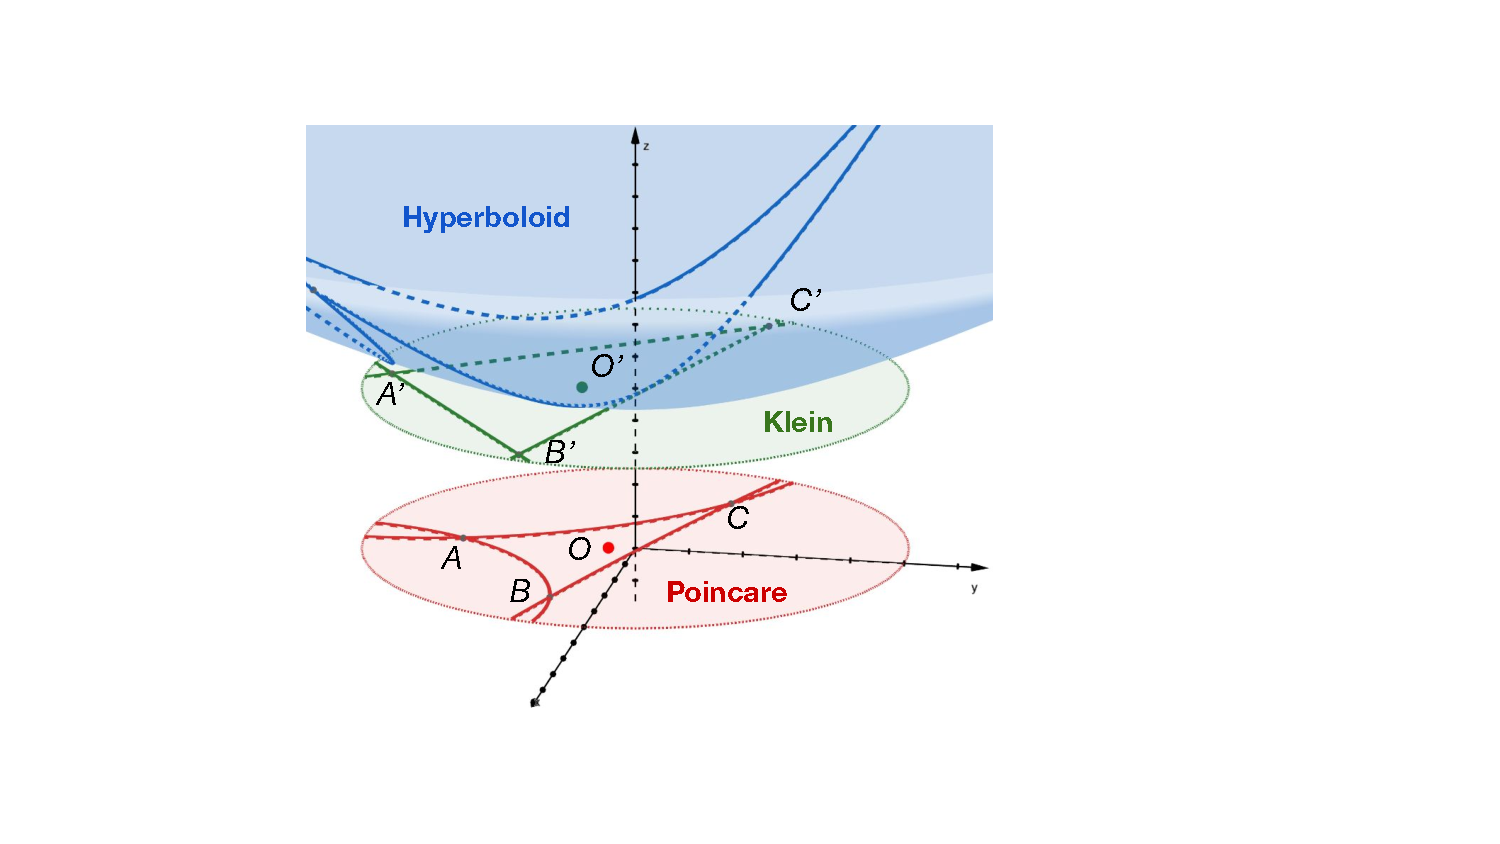
\includegraphics[width=.95\linewidth]{figures/hyperbolic.pdf}
\caption{Lines on different models for $2$-dimensional hyperbolic space.}
\vspace{-1em}
\label{fig:hyperbolic_models}
\end{wrapfigure}

Hyperbolic spaces are non-Euclidean spaces with negative curvature where given a fixed point and a line, there exist infinitely many parallel lines that can pass through this point. There are several commonly used isometric hyperbolic models \citep{cannon1997hyperbolic}. For this work, we mainly use the Poincaré Ball model. 

\begin{definition}[Manifold]
\label{eq:manifold}
A \textit{manifold} $\gM$ is a set of points $\vz$ that are locally Euclidean. Every point $\vz$ of the manifold $\gM$ is attached to a \textit{tangent space} $\gT_\vz \gM$, which is a vector space over the reals of the same dimensionality as $\gM$ that contain all the possible directions that can tangentially pass through $\vz$.
\end{definition}

\begin{definition}[\Poincare Ball Model] Given $c$ as a constant, the \Poincare ball model $(\sB_c^d,\mathfrak{g}_B)$ is defined by a manifold of an open ball $\sB_c^d=\{\vz\in\sR^d:c\|\vz\|^2< 1\}$ and metric tensor $\mathfrak{g}_B$ that defines an inner product of $\gT_\vz \sB_c^d$. The model is equipped with the distance \citep{ungar2001hyperbolic} as
\begin{equation}
d_{\sB_c}(\vz_1,\vz_2) = \frac{2}{\sqrt{c}}\tanh^{-1}\left(\sqrt{c}\left\lVert\frac{-(1 + 2c\left<-\vz_1, \vz_2\right> + c\|\vz_2\|^2)\vz_1 + (1 - c\|\vz_1\|^2)\vz_2}{1 - 2c\left<\vz_1,\vz_2\right> + c^2\|\vz_1\|^2\|\vz_2\|^2}\right\rVert\right).
\label{eq:poincaredistance}
\end{equation}
\end{definition}
For $c \to 0$, we can recover the properties of the Euclidean geometry since $\lim_{c \to 0} d_{\sB_c}(\vz_1,\vz_2) = 2\|\vz_1-\vz_2\|$. Since $\gT_\vz \sB_c^d$ is isomorphic to $\mathbb{R}^d$, we can connect vectors in Euclidean space and hyperbolic space with the bijection between $\gT_\vz \sB_c^d$ and $\sB_c^d$ \citep{ungar2001hyperbolic}. For $\vz = \mathbf{0}$, the \emph{exponential map} $\exp_\mathbf{0}^c : \gT_\vz \sB_c^d \to \sB_c^d$ and \emph{logarithm map} $\log_\mathbf{0}^c : \sB_c^d \to \gT_\vz \sB_c^d$ have the closed form of
\begin{equation}
\label{eq:hyp_maps}
    \exp_\mathbf{0}^c (\vv) = \tanh\left(\sqrt{c} \|\vv\| \right)\frac{\vv}{\sqrt{c}\|\vv\|}, \quad \log_\mathbf{0}^c (\vu) = \frac{1}{\sqrt{c}}\tanh^{-1}\left(\sqrt{c} \| \vu \| \right)\frac{\vu}{\|\vu \|}. 
\end{equation}
Alternatively, to guarantee the correctness of Poincaré distance computation, we can also process any Euclidean vector with a clipping module \citep{nickel2017poincare}
\begin{equation}
    \text{clip}^c(\vv) = \begin{cases}
			\vv, & \text{if $\|\vv\|< 1 / \sqrt{c}$}\\
                \left(\frac{1}{\sqrt{c}} - \epsilon\right) \frac{\vv}{\|\vv\|} , & \text{otherwise}
		 \end{cases},
\end{equation}
so the clipped vector is within the Poincare disk. We set $\epsilon$ as a small positive number in practice.

\begin{definition}[Klein Model]
Klein model $(\mathbb{K}_c^d, \mathfrak{g}_K)$ consists of an $1/\sqrt{c}$-radius open ball $\mathbb{K}_c^d = \{\vz\in\sR^d:c\|\vz\|^2 < 1\}$ and a metric tensor $\mathfrak{g}_K$ different from $\mathfrak{g}_B$. Similar to the mean computation in Euclidean space, let $\gamma_i = 1 / \sqrt{1 - c\|\vz_i\|^2}$, the Einstein midpoint of a group of Klein vectors $\vz_1, \dots \vz_n \in \mathbb{K}_c^d$ has a simple expression of a weighted average
\begin{equation}
    \text{HypAve}_K(\vz_1, \dots \vz_n) = \sum\limits_{i=1}^n \gamma_i \vz_i \bigg/ \sum\limits_{i=1}^n \gamma_i.
    \label{eq:hypave}
\end{equation}
\end{definition}
We illustrate the relationship between the different hyperbolic models in \Cref{fig:hyperbolic_models}. The hyperboloid space models $d$-dimensional hyperbolic geometry on a $d+1$-dimensional space. When $d = 2$, the Klein model is the tangent plane of the hyperboloid model at $(0,0,1)$, and the \Poincare disk shares the same support as the Klein disk, although shifted downwards and centered at the origin. Given a triangle on the hyperboloid model, its projection on the Klein model preserves the straight sides, but the projection of a line on the \Poincare model is a part of a circular arc or the diameter of the disk. Let $\vz_\mathbb{B}, \vz_\mathbb{K}$ be coordinates of $\vz$ under \Poincare and Klein model respectively, the prototype operations on $\mathbb{B}^d_c$ require transformations between $\mathbb{B}^d_c$ and $\mathbb{K}^d_c$ as
\begin{equation}
    \vz_\mathbb{B} = \frac{\vz_\mathbb{K}}{1 + \sqrt{1 - c\|\vz_\mathbb{K}\|^2}}, \quad \vz_\mathbb{K} = \frac{2\vz_\mathbb{B}}{1 + c\|\vz_\mathbb{B}\|^2}.
    \label{eq:Poincare2Klein}
\end{equation}
For example, in \Cref{fig:hyperbolic_models}, $O'$ is the $\text{HypAve}_\text{K}$ of $A',B',C'$, and can be mapped back to the \Poincare disk to get the \Poincare prototype ($\text{HypAve}_\text{B}$) $O$ of points $A, B, C$ by a change of coordinates.

\subsection{\texttt{HypStructure}: Hyperbolic Structured Regularization}
\label{sec:hypstructure-method}
At a high level, \texttt{HypStructure} uses a combination of two losses: a Hyperbolic Cophenetic Correlation Coefficient Loss (\texttt{HypCPCC})), and a Hyperbolic centering loss (\texttt{HypCenter}) for embedding the hierarchy in the representation space. Below we describe the two components of \texttt{HypStructure}. The pseudocode of \texttt{HypStructure} is shown in \Cref{alg:hypstructure} in \Cref{app:pseudocode}.


\textbf{HypCPCC (\underline{Hyp}erbolic \underline{C}o\underline{p}henetic \underline{C}orrelation \underline{C}oefficient):} We extend the $\ell_2$-CPCC methodology in \citet{zeng2022learning} to the hyperbolic space in \texttt{HypCPCC}. Three major steps of \texttt{HypCPCC} are (i) map Euclidean vectors to \Poincare space (ii)  compute class prototypes  (iii) use \Poincare distance for CPCC. Specifically, we first project each $\vz_i \in \mathbb{R}^d$ to $\mathbb{B}_c^d$, and compute the Poincaré centroid for each vertex of $\mathcal{T}$ using hyperbolic averaging as shown in \Cref{eq:hypave} and \Cref{eq:Poincare2Klein}. Alternatively, we can also compute Euclidean centroids $\overline{\vz} = \frac{1}{|\data_i|}\sum_{\vz \in \data_i}{\vz}$ for each vertex, and project each $\overline{\vz} \in \mathbb{R}^d$ to $\mathbb{B}_c^d$ either by $\exp_{\mathbf{0}}^c$ or $\text{clip}^c$. After the computation of hyperbolic centroids, we use the pairwise distances between all vertex pairs in $\mathcal{T}$ in the \Poincare ball, to compute the \texttt{HypCPCC} loss using \Cref{eq:CPCC} by setting $\rho = d_{\mathbb{B}_c}$. 

\textbf{HypCenter (\underline{Hyp}erbolic \underline{Center}ing):} Inspired by Sarkar's low-distortion construction \citep{Sarkar_2012} that places the root node of a tree at the origin, we propose a centering loss for this positioning, that enforces the representation of the root node to be close to the center of the \Poincare disk, and the representations of its children to be closer to the border of \Poincare disk. We enforce this constraint by minimizing the norm of the hyperbolic representation of the root node as $\ell_\text{center} = \norm{\text{HypAve}_B(\exp_{\mathbf{0}}^c(\vz_1), \dots, \exp_{\mathbf{0}}^c(\vz_N))}$. Alternatively, for centroids computed in the Euclidean space and mapped to the \Poincare disk, we minimize $\ell_\text{center} = \norm{1/N\sum_{i=1}^N f_\theta(\vx_i)}$ directly due to the monotonicity of $\tanh(\cdot)$ in the exponential map.

Finally, for $\alpha, \beta > 0$, we can learn the \emph{hierarchy-informed} representations by minimizing
\begin{equation}
    \label{eq:objective_hyp}
    \mathcal{L}(\data) = \sum_{(\vx, y)\in \data} \ell_\text{Flat}(\vx,y,\theta) - \alpha\cdot\hypcpcc(\tmetric, d_{\mathbb{B}_c}) + \beta \cdot\ell_\text{center}(\vx, \theta),
\end{equation}
where $\ell_\text{Flat}$ is a standard classification loss, such as the \texttt{CE} loss or the \texttt{SupCon} loss. 



\textbf{Time Complexity:} In a batch computation setting with a batch size $b$ and the number of classes (leaf nodes) as $k$, the computational complexity for a \texttt{HypStructure} computation to embed the full tree will still be $O(d\cdot\min\{b^2,k^2\})$, which is the same as the complexity of a Euclidean \emph{leaf-only} CPCC. The additional knowledge gained from internal nodes allows us to reason about the relationship between higher-level  concepts, and the hyperbolic representations help in achieving a low distortion of hierarchical information for better performance in downstream tasks.
